\documentclass{beamer}
%\usepackage[cp866]{inputenc}
\usepackage[utf8x]{inputenc}
%\usepackage[koi8-r]{inputenc}
%\usepackage[russian]{babel}
\usepackage[russian]{babel}
\usepackage{pgf,pgfarrows,pgfnodes,pgfautomata,pgfheaps,pgfshade}
\usepackage{beamerthemesplit}
\usepackage{rotate}
%\usepackage[euler]{textgreek}
\usepackage{bm}
\usepackage{amssymb,amsmath,amscd,epsfig}
%\usepackage[dvips]{color}
\usepackage{lscape}
\usepackage{epsfig}
\usepackage{graphicx}
\usepackage{color}
\usepackage{caption}
%\usepackage{axodraw}
\usepackage{amsmath}
\usepackage{amssymb}
\usepackage{verbatim}
\usepackage{hyperref}
\usepackage{algorithm,algorithmic}
\usetheme{Rochester}
\setbeamercolor{background canvas}{bg=green!0}
\definecolor{colorone}{rgb}{0.0,0.35,0.35}
\definecolor{colortwo}{rgb}{0.0,0.0,0.35}
\definecolor{colorthree}{rgb}{0.85,0.0,0.0}
\definecolor{colorfour}{rgb}{0.05,0.56,0.05}
\definecolor{colorfive}{rgb}{1.0,0.18,0.92}
\definecolor{colorsix}{rgb}{0.5,0.188,0.0}

\title
{Поиск кратчайших путей между всеми вершинами графа}
\author{Д.А.~Арбузова, Э.А.~Зиннурова, О.П.~Найдин, О.А.~Харациди}
\date{\today}
\begin{document}
%---------------------------------------------------------------------------------------------------------------------------------------------------------01
\frame{\titlepage}
%---------------------------------------------------------------------------------------------------------------------------------------------------------02
\frame{
\frametitle {Постановка задачи}
Ориентированный взвешенный граф $G = (V, E), |V| = N,$ задан своей матрицей смежности $A = (a_{ij})_{N\times N},$ где
\small
$$
a_{ij} = \begin{cases}
		\text{вес ребра из вершины $i$ в вершину $j$, если таковое имеется},\\
		\infty \text{ иначе}.
		\end{cases}
$$\\
\normalsize
Требуется определить кратчайшие расстояния между каждой парой вершин графа.
}

\frame{
\frametitle {Алгоритм решения}
Для решения поставленной задачи воспользуемся алгоритмом Флойда --- Уоршелла.\\
\begin{algorithm}[H]
	\begin{algorithmic}[1]
		\FOR{$k=1$ to $N$}
			\FOR{$i=1$ to $N$}
				\FOR{$j=1$ to $N$}
					\STATE $a_{ij} = \min(a_{ij}, a_{ik} + a_{kj})$
				\ENDFOR
			\ENDFOR
		\ENDFOR
	\end{algorithmic}
	\caption{Псевдокод алгоритма Флойда}
	\label{alg:seq}
\end{algorithm}
Сложность алгоритма: $O(N^3).$
}

\frame{
\frametitle {Варианты распараллеливания}
\begin{minipage}{0.55\textwidth}
\begin{algorithm}[H]
	\begin{algorithmic}[1]
		\FOR{$k=1$ to $N$}
			\FOR{$i=i_{\text{local start}}$ to $i_{\text{local end}}$}
				\FOR{$j=1$ to $N$}
					\STATE $a_{ij} = \min(a_{ij}, a_{ik} + a_{kj})$
				\ENDFOR
			\ENDFOR
		\ENDFOR
	\end{algorithmic}
	\caption{Распараллеливание по одной размерности матрицы $A$}
	\label{alg:seq}
\end{algorithm}
\end{minipage}
\begin{minipage}{0.4\textwidth}
\vspace{30pt}
\begin{figure}[H]
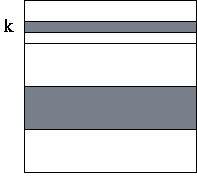
\includegraphics[width=\textwidth]{./par1.png}
\end{figure}
\vspace{10pt}
\end{minipage}
Максимальное число процессов: $N.$
}

\frame{
\frametitle {Варианты распараллеливания}
\begin{minipage}{0.55\textwidth}
\begin{algorithm}[H]
	\begin{algorithmic}[1]
		\FOR{$k=1$ to $N$}
			\FOR{$i=i_{\text{local start}}$ to $i_{\text{local end}}$}
				\FOR{$j=j_{\text{local start}}$ to $j_{\text{local end}}$}
					\STATE $a_{ij} = \min(a_{ij}, a_{ik} + a_{kj})$
				\ENDFOR
			\ENDFOR
		\ENDFOR
	\end{algorithmic}
	\caption{Распараллеливание по двум размерностям матрицы $A$}
	\label{alg:seq}
\end{algorithm}
\end{minipage}
\begin{minipage}{0.4\textwidth}
\vspace{30pt}
\begin{figure}[H]
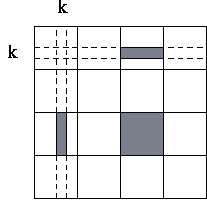
\includegraphics[width=\textwidth]{./par2.png}
\end{figure}
\vspace{10pt}
\end{minipage}
Максимальное число процессов: $N^2.$
}

\frame{
\frametitle {Генерация графа}
Выберем $N$ и будем генерировать матрицу $А$ следующим образом:
$$
a_{ij} = \begin{cases}
		\text{rand}(1000), p\\
		\infty, 1 - p,
		\end{cases}
$$
где $p$ --- вероятность образования ребра.\\
Поскольку сложность алгоритма зависит от $N = |V|,$ а не от $|E|,$ то большой роли значение $p$ не играет.
}

\frame{
\frametitle {Эксперименты}
Проведём эксперименты для различных параметров $N$ и числа потоков $K$, измеряя время работы параллельной программы.\\
$N = 10^i, i = \overline{1, 5}$ ?\\
$K = 2^i, i = \overline{1, 5}$ ?
}

\frame{
\frametitle {Эксперименты. MPI}
График speedup
\begin{table}[H]
\begin{tabular}{|c|c|c|}
\hline
Число потоков & Время работы, с & Ускорение\\
\hline
\end{tabular}
\end{table}
}

\frame{
\frametitle {Эксперименты. Hybrid}
График speedup
\begin{table}[H]
\begin{tabular}{|c|c|c|}
\hline
Число потоков & Время работы, с & Ускорение\\
\hline
\end{tabular}
\end{table}
}

\frame{
\frametitle {Использованные источники}
\href{http://www.mcs.anl.gov/~itf/dbpp/text/node35.html}{http://www.mcs.anl.gov/~itf/dbpp/text/node35.html}\\
\href{http://www.academia.edu/243222/An\_Investigation\_Of\_Different\_Hybrid\_OpenMp\_and\_MPI\_Implementations\_Of\_Floyds\_All-Pairs-Shortest-Path\_Algorithm}{http://www.academia.edu/243222/An\_Investigation\_Of\_Different\_Hybrid\_OpenMp\_and\_MPI\_Implementations\_Of\_Floyds\_All-Pairs-Shortest-Path\_Algorithm}
}
\end{document}